% !TeX root = ..\main.tex
\section{Cơ sở lý thuyết}
\subsection{Lược đồ BPMN}
\subsubsection{Tổng quan về BPMN}

\hspace*{0.5cm}BPMN(Business Process Modeling Notation) là một lược đồ tập hợp các kí hiệu để mô hình hóa trực quan các quy trình nghiệp vụ xử lý . BPMN giúp các doanh nghiệp trực quan hóa các hoạt động và các luồng thông tin để thực hiện quy trình nghiệp vụ.
\begin{figure}[!htp]
	\centering
	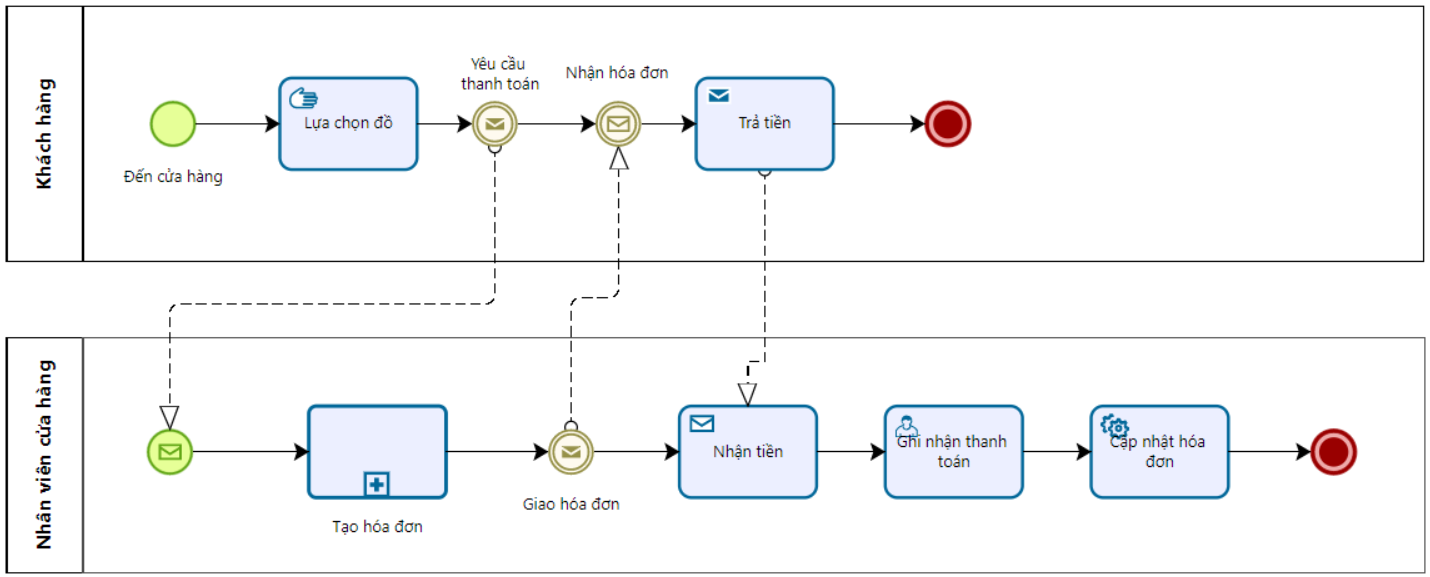
\includegraphics[width=10cm]{img/theory/BPMN/BPMN_sample.png}
	\newline
	\caption{Ví dụ về lược đồ BPMN}
\end{figure}



\subsubsection{Lợi ích của BPMN}
\begin{itemize}
	\item Giúp các bên liên quan có thể hiểu rõ quy trình nghiệp vụ của hệ thống
	\item Thu hẹp khoảng cách giửa bộ phận thiết kế và bộ phận nghiệp vụ
	\item Dễ dàng mô tả các nghiệp vụ phức tạp
\end{itemize}

\subsubsection{Các thành phần của BPMN}
\subsubsubsection*{Swimlane}
Swimlane bao gồm Pool và Lane:
\begin{itemize}
	\item Pool: Đại diện cho một tổ chức, phòng ban, một vai trò hoặc một hệ thống nào đó.
	\item Lane: Đại diện các cá nhân riêng lẻ, người sẽ làm các hoạt động cụ thể.
\end{itemize}

\begin{figure}[!htp]
	\centering
	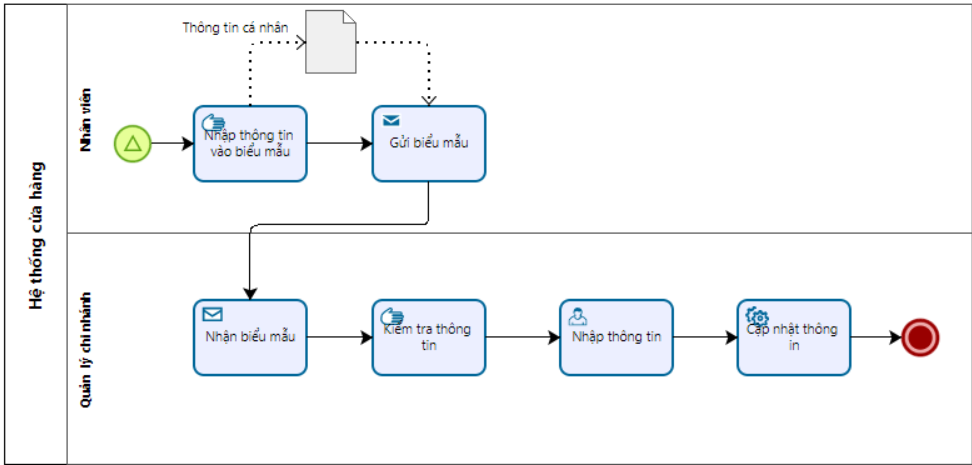
\includegraphics[width=10cm]{img/theory/BPMN/BPMN_swimlane.png}
	\newline
	\caption{Lược đồ BPMN bao gồm 1 pool(Hệ thống cứa hàng) và 2 lane (Nhân viên, Quản lý chi nhánh)}
\end{figure}

\subsubsubsection*{Activities}
Mô tả công việc trong quy trình, được kí hiệu bằng một kình chử nhật bo tròn 4 góc. Bao gồm 4 loại:
\begin{itemize}
	\item Task: Các việc nhỏ, đơn lẻ
	      \begin{figure}[!htp]
		      \begin{center}
			      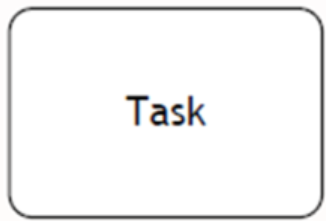
\includegraphics[width=2cm]{img/theory/BPMN/Task.png}
		      \end{center}
		      \caption{Task}
	      \end{figure}
	\item Event Sub-Process: Một quy trình con nằm trong một quy trình lớn, chức nhiều task
	      \begin{figure}[!htp]
		      \begin{center}
			      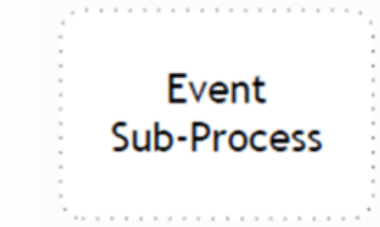
\includegraphics[width=2cm]{img/theory/BPMN/Event Sub-process.png}
		      \end{center}
		      \caption{Event Sub-Process}
	      \end{figure}
	\item Transaction: Các giao dịch, bao gồm các task nhỏ khác logic với nhau
	      \begin{figure}[!htp]
		      \begin{center}
			      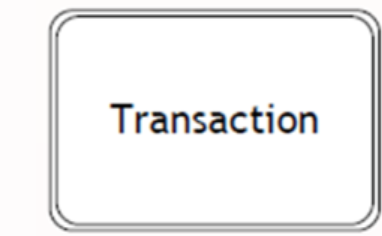
\includegraphics[width=2cm]{img/theory/BPMN/Transaction.png}
		      \end{center}
		      \caption{Transaction}
	      \end{figure}
	\item Call Activity: Gọi một quy trình khác đã được định nghĩa trong hệ thống, thay vì phải định nghĩa lại nhiều lần
	      \begin{figure}[!htp]

		      \begin{center}
			      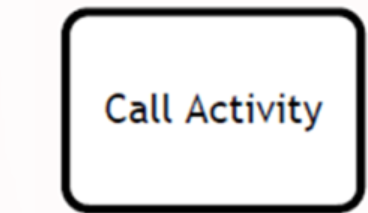
\includegraphics[width=2cm]{img/theory/BPMN/Call Activity.png}
		      \end{center}
		      \caption{Call Activity}
	      \end{figure}
\end{itemize}
\begin{flushleft}
	Các hình ảnh được lấy từ \url{https://thinhnotes.com/chuyen-nghe-ba/giai-ngo-cac-ky-hieu-bpmn/}
\end{flushleft}


\subsubsubsection*{Events}
Sự kiện là một điều gì đó xảy ra và có thể tác động đến quy trình nghiệp vụ. Một sự kiện có thể là bên ngoài hoặc bên trong nội bộ. Miễn là nó có tác động và ảnh hưởng trực tiếp đến quy trình nghiệp vụ. Các sự kiện thường được kí hiệu bằng hình tròn, bên trong có các kí hiệu về loại hình kích hoạt. Bao gồm các loại:
\begin{itemize}
	\item Start: Các sự kiện mở đầu quy trình nghiệp vụ
	\item Intermediate: Các sự kiện xảy ra giữa các quy trình nghiệp vụ
	\item End: Các sự kiện kết thúc quy trình nghiệp vụ
\end{itemize}
\begin{figure}[!htp]
	\begin{center}
		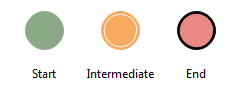
\includegraphics[width=6cm]{img/theory/BPMN/Event.png}
	\end{center}
	\caption{Các loại sự kiện trong BPMN}
\end{figure}
\begin{flushleft}
	Hình ảnh được lấy từ \textit{\url{https://www.edrawsoft.com/what-is-bpmn.html?gclid=Cj0KCQiAvqGcBhCJARIsAFQ5ke5U9xsSqU24T_1MgVtsStQ3wV0NbkzXcIY-rDCU8JAet5rGQMc6PyIaAgdxEALw_wcB}}
\end{flushleft}



\subsubsubsection*{Gateways}
Các cổng có nhiệm vụ chính là kiểm soát dòng chảy của quy trình nghiệp vụ. Cổng thường kí hiệu hình thoi, bên trong là kí hiệu các loại.
\begin{itemize}
	\item Start: Các sự kiện mở đầu quy trình nghiệp vụ
	\item Intermediate: Các sự kiện xảy ra giữa các quy trình nghiệp vụ
	\item End: Các sự kiện kết thúc quy trình nghiệp vụ
\end{itemize}
\begin{figure}[!htp]
	\begin{center}
		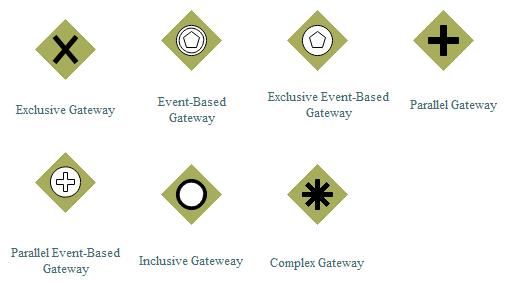
\includegraphics[width=8cm]{img/theory/BPMN/Gateway.png}
	\end{center}
	\caption{Các loại cổng phổ biến trong BPMN}
\end{figure}
\begin{flushleft}
	Hình ảnh được lấy từ \url{https://www.bacs.vn/vi/blog/kien-thuc/tong-quan-ve-bpmn-danh-cho-business-analyst-11002.html}
\end{flushleft}



%%%%%%%%%%%%%%%%%%%%%%%%%%%%%%%%%
\subsection{Ngôn ngữ BPEL}
\subsubsection{Tổng quan về BPEL}
\hspace*{0.5cm} BPEL hay BPEL4WS(Business Process Execution Language for Web Services) là ngôn ngữ dùng để định nghĩa và thực thi các quy trình nghiệp vụ sử dụng các dịch vụ web. Ngôn ngữ BPEL được xây dựng dựa trên nền tảng XML hỗ trợ các dịch vụ web: SOAP, WSDL, UDDI. BPEL xây dựng một dịch vụ web dựa trên việc điều phối, phối hợp các dịch vụ web độc lập khác để hình thành nên một dịch vụ web mới.
\subsubsection{Các thành phần trong BPEL}
BPEL bao gồm các thành phần nguyên tố và các thành phần cấu trúc. Các thành phần nguyên tố bao gồm:
\begin{itemize}
	\item $<invoke>$: Gọi một dịch vụ web khác
	\item $<receive>$: Đợi phản hồi tự các tác vụ bất đồng bộ
	\item $<reply>$: Phản hồi cho các tác vụ đồng bộ
	\item $<assign>$: Gán giá trị cho biến
	\item $<throw>$: Chỉ định các lỗi, ngoại lệ
	\item $<wait>$: Đợi một thời gian
	\item $<terminate>$: Kết thúc toàn bộ quy trình
\end{itemize}

Bên cạnh thành nguyên tố, các thành phần cấu trúc chứa nhiều tác vụ bên trong:
\begin{itemize}
	\item $<sequence>$: Các tác vụ thực hiện tuần tự
	\item $<flow>$: Các tác vụ thực hiện song song
	\item $<switch>$: Thực hiện các tác vụ rẽ nhánh
	\item $<while>$: Thực hiện các vọng lặp
\end{itemize}

Ngoài ra, còn có $<partnerLink>$ dùng để xác định các đối tác, các dịch vụ web sử dụng, $<variable>$ để định nghĩa các biến cần thiết trong quy trình


\subsubsection{Ví dụ về BPEL}

\hspace*{0.5cm} Để hiểu rõ về quy trình được mô tả bằng BPEL, ta xem xét ví dụ về quy trình sắp xếp chuyến đi cho nhân viên. Đầu tiên, chúng ta sẽ kiếm tra hạng vé của nhân viên, giả sử rằng có một dịch vụ web Employee Travel sẽ làm việc này. Sau đó, chúng ta kiểm tra giá vé của hai hãng: American Airlines và Delta Airlines để chọn ra giá vé thấp hơn và trả lại kết quả. Quy trình này được minh họa như sau:

\begin{figure}[!htp]
	\begin{center}
		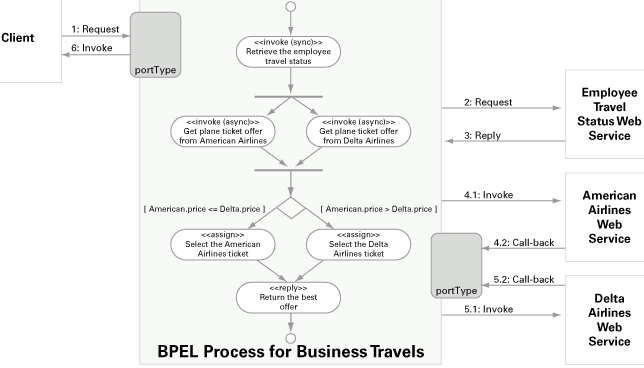
\includegraphics[width=10cm]{img/theory/BPEL/Sample.png}
	\end{center}
	\caption{Ví dụ về quy trình BPEL sắp xếp chuyến đi}
\end{figure}

\begin{flushleft}
	Hình ảnh được lấy từ \url{https://www.oracle.com/technical-resources/articles/matjaz-bpel.html}
\end{flushleft}

Trong ví dụ này, các partner của hệ thống sẽ bao gồm Client, Employee Travel Status Web Service, American Airlines Web Service, Detal Airlines Web Service. Chúng ta sẽ xây dựng một quy trình BPEL bất đồng bộ, giả định rằng dịch vụ web Employee Travel là đồng bộ vì dữ liệu nhân viên đã có sẵn và có thể phản hồi ngay lập tức. 

Quy trình BPEL chi tiết như sau: Đầu tiên Client sẽ gửi một yêu cầu bất đồng bộ kèm theo thông tin chuyến đi đến hệ thống. Hệ thống sẽ nhận thông tin và thực hiện lệnh gọi đồng bộ sang dịch vụ web Employee Travel để lấy thông tin hạng vé của nhân viên này. Tiếp theo, hệ thống sẽ thực hiện 2 lệnh gọi bất đồng bộ đồng thời đến 2 dịch vụ web của American Airlines và Delta Airlines để xác định giá vé. Sau khi hệ thống nhận được phản hồi kết quả của 2 hãng hàng không, hệ thóng thực hiện so sánh để tìm giá vé thấp hơn và trả lại kết quả cho Client. Quy trình kết thúc. 

\subsubsection{Các bước xây dựng quy trình BPEL}
Để xây dựng ví dụ trên, ta cần thực hiện các bước sau:
\begin{enumerate}
	\item Xác định các dịch vụ web liên quan: Xác định các dịch vụ web tương tác đối với hệ thống (Employee Travel Web Service, American Airlines Web Service, Delta Airlines Web Service)
	\item Xây dựng WSDL cho quy trình BPEL: BPEL là một dịch vụ web, do đó ta cần xây dựng WSDL cho chính nó
	\item Xác định partnerLink cho quy trình: Cần xác định các dịch vụ web được thực hiện đồng bộ hay bất đồng bộ, cần những tham số nào để gọi.
	\item Xây dựng quy trình: Xây dựng các luồng đi, logic trong quy trình
\end{enumerate} 


%%%%%%%%%%%%%%%%%%%%%%%%%%%%%%%%%
\subsection{Chuyển đổi BPMN sang BPEL}